\section{}

\begin{quote}
	The National Transportation Safety Board determines that the probable cause of the pipeline rupture was a pressure surge initiated by the automatic shutdown of a pump station caused by the dispatcher's delay in getting it started, followed by his attempt to relieve the surge pressure into a stub-line connection instead of following the company procedure of shutting down all of the pumps on the line \citep{NTSB1981}.
\end{quote}

\begin{quote}
	[T]he NTSB concludes that although Enbridge had procedures that required a pipeline shutdown after 10 minutes of uncertain operational status, Enbridge control center staff had developed a culture that accepted not adhering to the procedures \citep{NTSB2012}.
\end{quote}

The pipeline industry in the US and its regulator have made great efforts over the last 40 years to improve pipeline safety, cutting the spill volume per barrel-mile transported more than in half (see Figure 1).\footnote{A barrel-mile is one barrel of oil transported over one mile. Hence, ten gallon-miles could describe either one gallon transported over ten miles, or ten gallons transported over one mile. This method of standardizing oil transport has the advantage that it takes into consideration both the extend, and utilization of a pipeline network.} Yet, a 1970s critic of the Trans-Alaska Pipeline System would be as correct as a current critic of the currently planned Keystone XL pipeline in saying this infrastructure remains inherently dangerous. Since the turn of the millenium, in the area of refined petroleum pipelines, efforts to make pipelines more safe have bottomed out, and gains in the safety of crude pipelines have been offset by a growth of the network and increase of utilization. In other words, there are more pipelines, therefore, there are more spills. Is it possible at all to remove the risks of environmental damages from a technology with catastrophic potential? \textit{What are the limits to organizational and population level learning?}

\noindent{==================================================
	\centerline{Insert Figure 1 about here}
	==================================================}
\begin{figure}
	\caption{Pipeline safety improvements at the industry level}
	\centerline{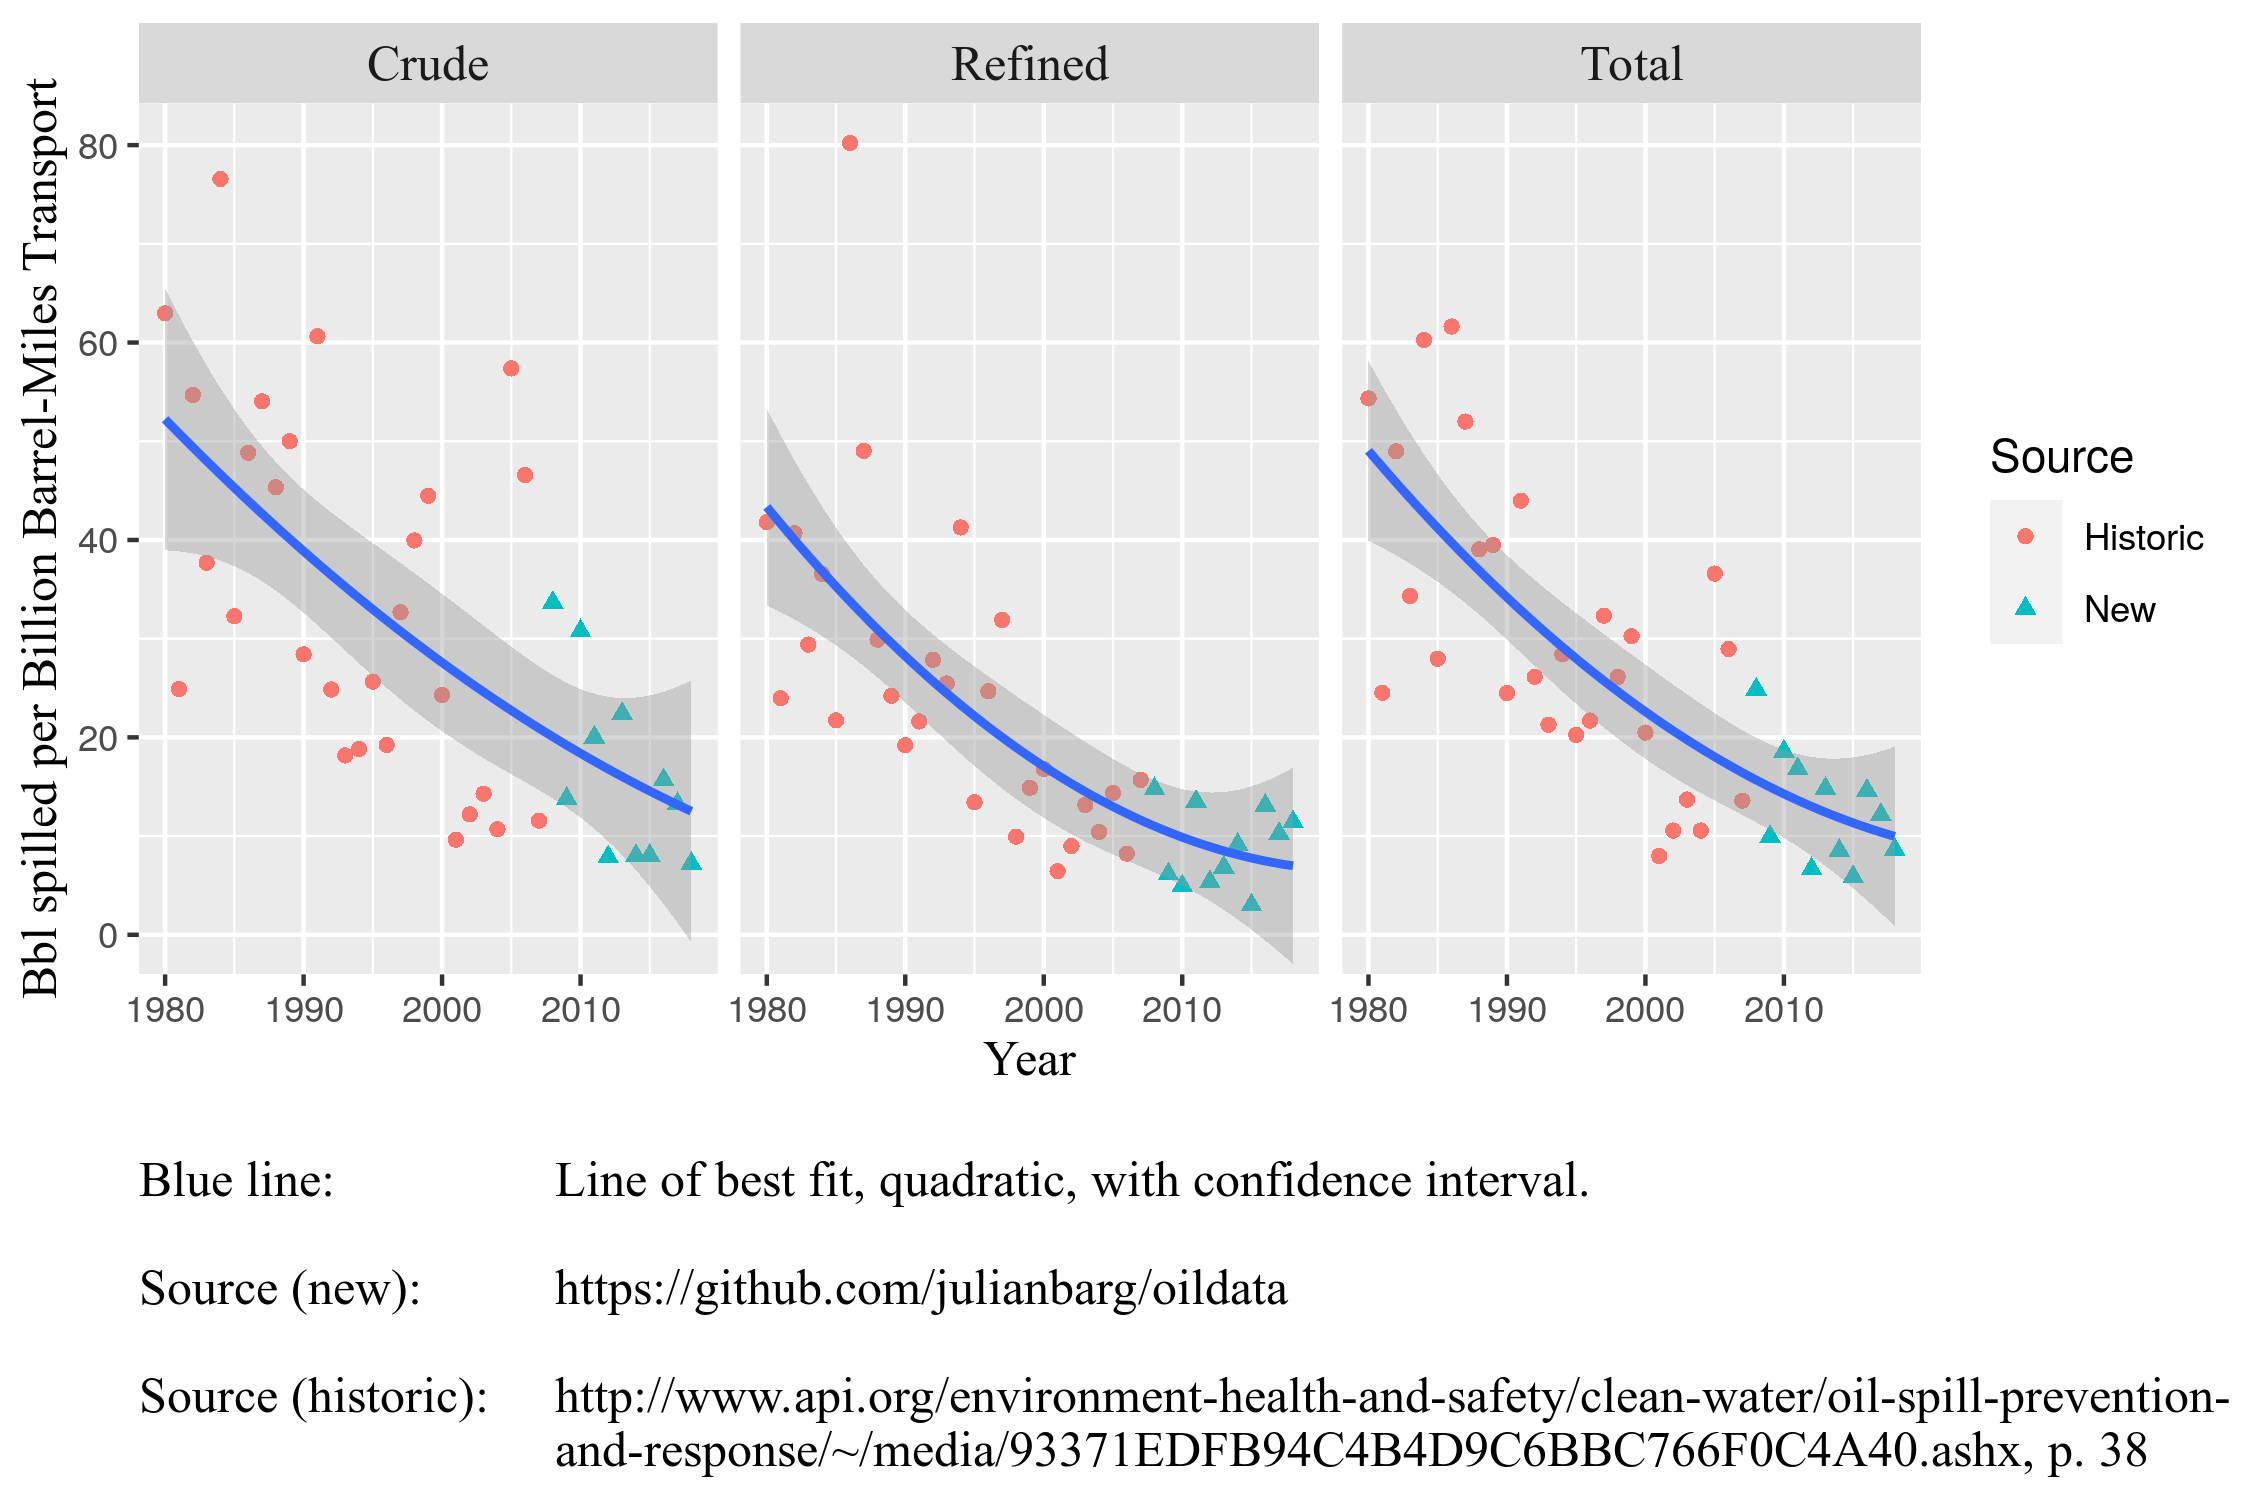
\includegraphics{../illustrations/population_learning_4.png}}
\end{figure}

Convergence of organizational learning efforts has been observed as early as the 1930s \citep{Wright1936}. Argote summarizes this literature: "As organizations produce more of a product, the unit cost of production typically decreases at a decreasing rate" \citep[p. 1]{Argote2013-1}, and this relationship (the \textit{learning curve}) has been found to hold for many other outcome variables that organizations care about. The relationship between experience and unit cost is great news for organizations that seek to increase profits. However, the notion that there is a limit to to this relationship could spell bad news  with regard to environmental pollution.

With dissertation, I contribute (1) to the literature on \textit{grand challenges} \citep{George2016}. I am taking stock on the current levels of chemical pollution caused by the pipeline industry. Chemical pollution is identified as one of the nine areas of human impact that potentially infringes on our planet's safe operating boundaries \citep{Rockstrom2009a}. The effort to explore management of environmental pollution is motivated by a call of \citet{George2015} for an investigation of theories of technology adoption and their implications for our use of decreasing natural capital. (2) In service of discussing resource use, this dissertation reconnects existing knowledge on the behavior of organizations \citep{March1963}, with more recent developments in organizational learning. In particular, \citet{Levitt1988} propose a model of organizational learning that goes beyond the learning curve \textit{and} derived theories that seek to decompose learning \citep[e.g.,][p. 2]{Argote2013-1}. Relevant for the phenomenon at hand, the authors conclude that "[t]he same processes that that yield experiential wisdom produce superstitious learning, competency traps, and erroneous inferences" \citep[p. 335]{Levitt1988}, and propose ways to address these issues. This dissertation talks to the limits of organizational and population level learning, with that cautious note in mind.

This dissertation employs both quantitative and qualitative data. (1) The first chapter juxtaposes qualitative evidence for learning past the turn of the millenium with a bottomed out or leveled off learning curve (where learning proceeds only at a very slow pace) for refined petroleum pipelines. What leads to a learning curve bottoming out in that fashion? The quantitative data available on the pipeline industry includes the extent of individual pipeline operators' networks, and the pipeline spills stemming from those networks. This data also allows us to track the elimination of certain spill types. The qualitative archival data reveals the complexity and interactions that lead to pipeline spill (such as staff not always following procedures, as exemplified by the introductory quotes), which are difficult to eliminate. (2) The second chapter combined two different literatures on learning to lay out the theoretical underpinnings of the bottoming out process. (3) The third chapter uses qualitative data to analyze the microfoundations of learning bottoming out.